\documentclass[runningheads,a4paper]{llncs}
\usepackage{amssymb}
\setcounter{tocdepth}{3}
\usepackage{graphicx}
\usepackage{csquotes}
\usepackage{xcolor, color}

\usepackage{url}
\newcommand{\keywords}[1]{\par\addvspace\baselineskip
\noindent\keywordname\enspace\ignorespaces#1}


%%%%%%%%%%%%%%%%%%%%%%%%%%%%%%%%%%%%%%%%%%%%%%%%%%%%%%%%%%%%%%%%%%%%%%%%%%
%%%%%%%%%%%%%%%%%%%%%%%%%%%%%%%%%%%%%%%%%%%%%%%%%%%%%%%%%%%%%%%%%%%%%%%%%%
%%%%%%%%%%%%%%%   TODO & COMMENTS
\usepackage{todonotes}

\newif\ifdraft\drafttrue % Change to \draftfalse% for removing comments
\ifdraft
   \newcommand\todos[1]{\medskip\todo[inline]{TODO (all): #1}}
   \newcommand\moussa[1]{\medskip\todo[color=green!40,inline]{\textbf{Moussa ---} \protect{#1}}}
   \newcommand\amanuel[1]{\medskip\todo[color=blue!40,inline]{\textbf{Amanuel ---} #1}}
   \newcommand\vincent[1]{\medskip\todo[color=green!40,inline]{\textbf{Vincent ---} #1}}
   \newcommand\abdel[1]{\medskip\todo[color=green!40,inline]{\textbf{Abdel ---} #1}}
\else
   \newcommand\todos[1]{}
   \newcommand\moussa[1]{}
	\newcommand\amanuel[1]{}
	\newcommand\vincent[1]{}
	\newcommand\abdel[1]{}
\fi
%%%%%%%%%%%%%%%%%%%%%%%%%%%%%%%%%%%%%%%%%%%%%%%%%%%%%%%%%%%%%%%%%%%%%%%%%%


\begin{document}

\mainmatter  % start of an individual contribution

\title{Interoperability at the Application Layer in the Internet of Things}
\titlerunning{}

\author{
Abdelmounaim DEBIECHE \and 
Moussa Amani \and
Vincent Englebert }
%
\authorrunning{Interoperability at the Application Layer in the Internet of Things}
% (feature abused for this document to repeat the title also on left hand pages)

\urldef{\mailsa}\path|{Abdelmounaim.Debieche,Moussa.Amrani, Vincent.Englebert}@unamur.be|

  

\institute{University of Namur, PReCISE Research Center, Belgium\\
\mailsa \\ 
Vrije Universiteit Brussel\\
 ETRO, Belgium\\
\mailsb}

\toctitle{An MDE Approach for the Well-Being of Ageing People}
%\tocauthor{Authors' Instructions}



\def\textem#1{\emph{#1}}
%Abstract
\subsection{General Architecture}
\label{sec:CG-Architecture}

Our proposal relies on a middleware that embeds a \CEP engine for handling event processing, as depicted in Figure \ref{fig:Architecture}. Our tool offers a simulation mode, where devices are simulated as software components mimicking their actual execution, thus allowing to test \IOT scenarios without physical devices.

\begin{figure}%
	\centering  
	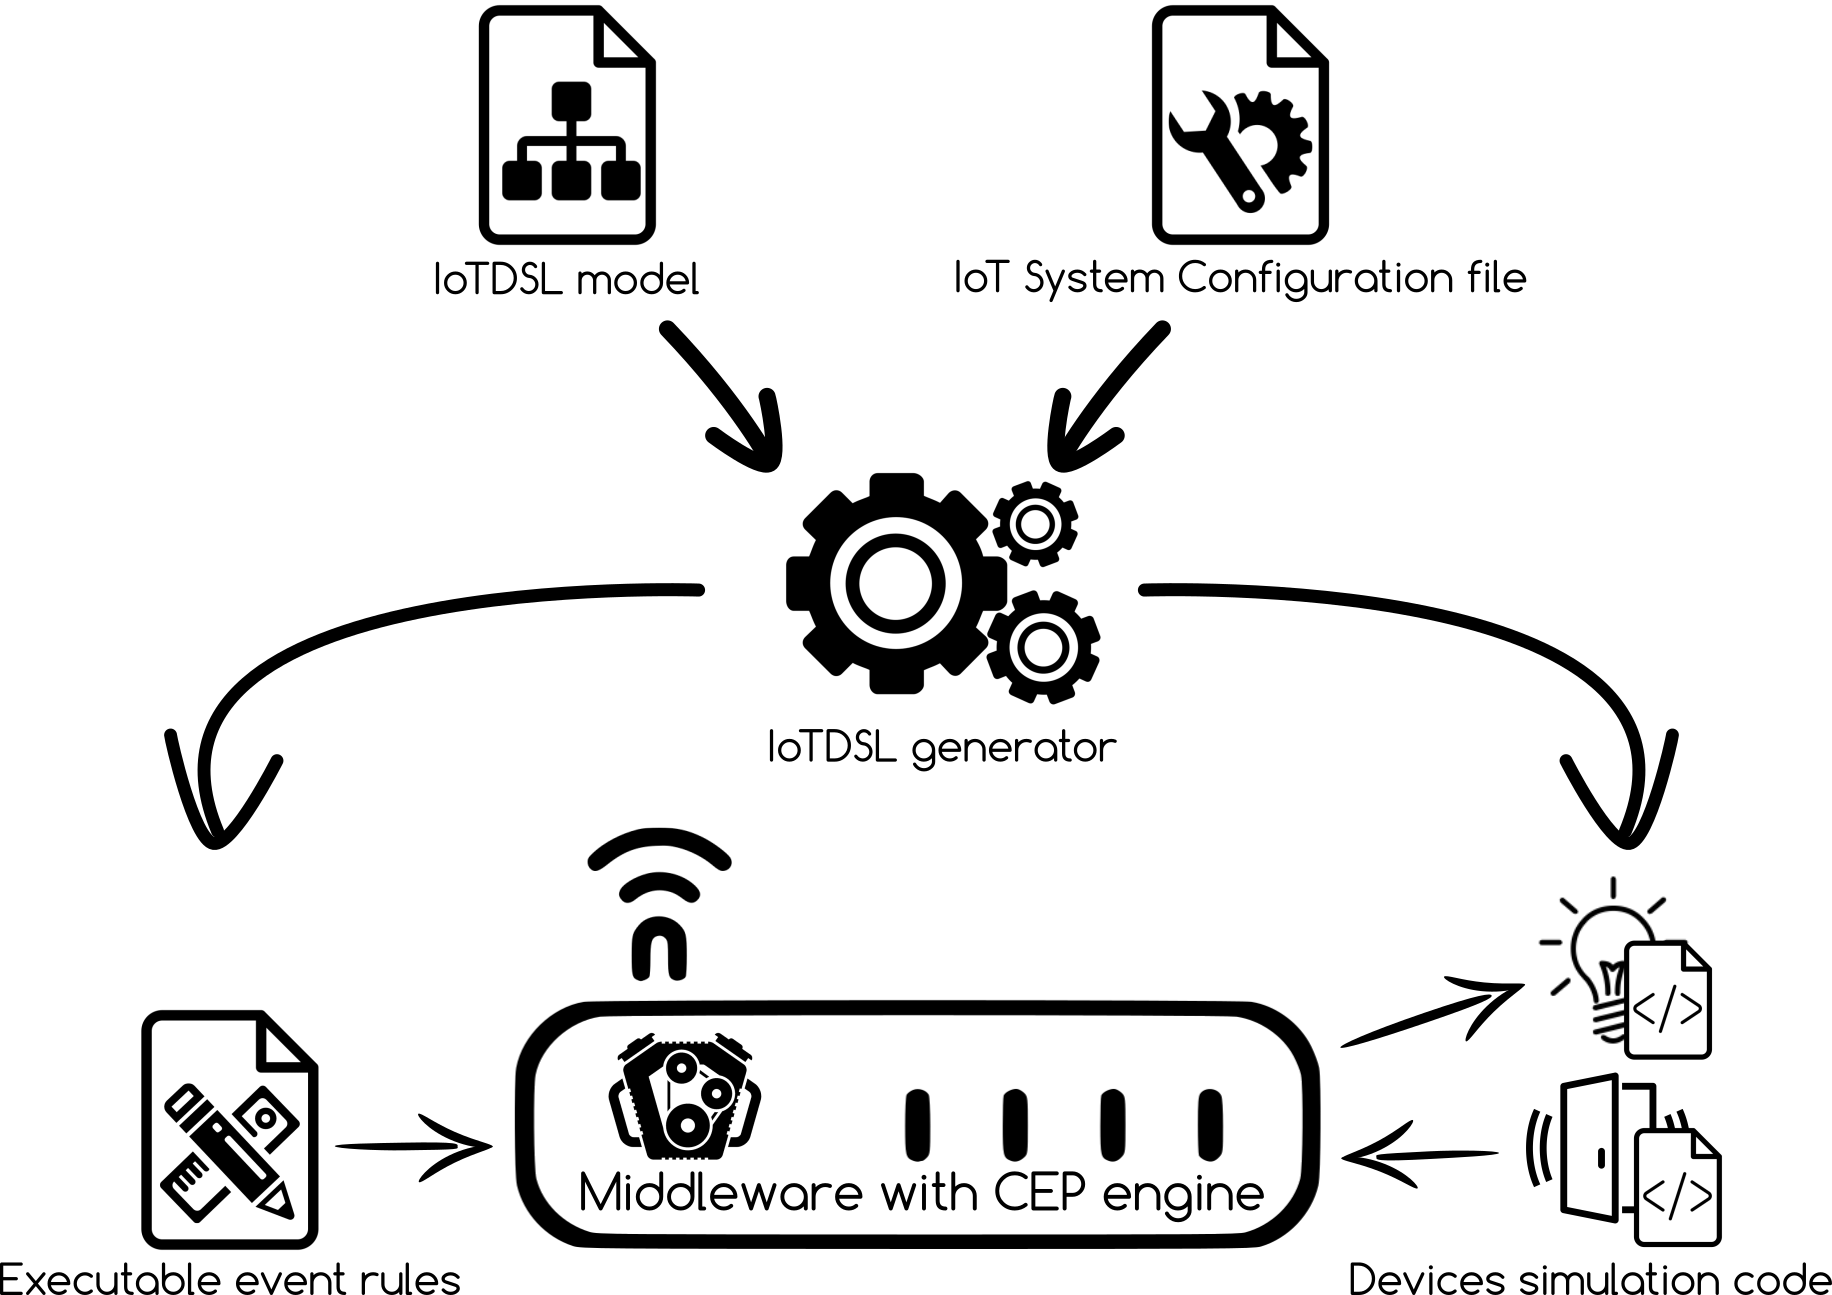
\includegraphics[width=.9\linewidth]{gen-archi.png}%
	\caption{General architecture of \IOTDSL framework}%
	\label{fig:Architecture}%
\end{figure}

The central element is the automatic code generator process: it produces executable code from \IOTDSL models and configuration files that define platform-specific details on the execution timing of devices (that the technicians set once and for all), and, for the purpose of our prototype, simulation code used to emulate the behaviour of the devices. The executable code is deployed into the \CEP engine running on a middleware, which reuses in simulation mode the simulation code for communicating with the (abstract) devices. 

%From \IOTDSL models, the generator will create a set of files that gather, on the one side, all rules as executable complex events and on the other side, a set of simulation code used to emulate the devices' behaviours. The event rules will be deployed in a \CEP engine running on a middleware and the individual simulation files will be used to test the whole infrastructure.

We are currently investigating how business rules could be broken down into smaller clusters that could be deployed directly into devices, assuming they present sufficient battery and computing power. When addressing non-functional properties of devices, we envision the possibility of expressing technical specifications relative to the energy consumption and computation capabilities of devices in a separate file that \IOTDSL would take into consideration for identifying distributable rules.

%As we already mentioned, at present time the rules are all gathered and managed by a centralised entity where the simulation files are each emulating a single device. We are currently investigating how all business rules can be split into smaller chunks to be run on devices themselves when those objects have sufficient battery and CPU power. As we are developing the non-functional properties for \IOTDSL type and mapping definitions, those characteristics will be expressible in the form of technical specifications for devices and thus powerful equipments that are meeting some minimum requirements will be identified as deployment targets for distributed \CEP engines. 

\section{Application Protocols}
\label{sec:Methodology}



\section{Related Work}
\label{sec:OO}





\bibliographystyle{splncs03}
\bibliography{./bibfile}
\end{document}
